%\newpage
\section{Messung von Halbleitern}
Ein Testpin wird als negative Seite des Bauteils angenommen.
Ein anderer Pin wird als positive Seite des Bauteils angenommen.
Als erster Test wird die positive Seite des Bauteils direkt mit VCC verbunden.
Die negative Seite wird mit dem \(680\Omega\) Widerstand nach GND verbunden.
Der Testpin (dritter Pin, auch TriStatePin genannt) wird zuerst mit dem \(680\Omega\)-Widerstand
für 10ms mit GND verbunden.
Die Spannung des negativen Testpins wird gemessen, während der TriStatePin auf Eingang
geschaltet ist.
Es wird angenommen, dass das getestete Bauteil ein P-Kanal-MOSFET sein kann und dass das Gate
entladen sein sollte.
Wenn die gemessene Spannung über 976mV ist, nimmt der nächste Test an. dass das getestete
Bauteil auch ein P-Kanal-MOSFET sein könnte und dafür wird der \(680\Omega\) Widerstand
für 10ms zur VCC-Seite geschaltet.
Auch für diesen Fall wird die Spannung des negativen Pins mit stromlosen TriStatePin gemessen.
Wenn die Spannung des negativen Pins grösser als 455mV ist, werden zusätzliche Tests gemacht, 
um N-Kanal JFET oder D-MOSFET (Verarmungs-Typ) und P-Kanal JFET oder P-MOSFET zu unterscheiden.
Die MOSFET-Versionen können erkannt werden durch das Fehlen von Steuerstrom in jedem 
TriStatePins Zustand.

Um Parameter der Verarmungstypen messen zu können, werden sie mit einem \(680 \Omega\)-Widerstand am
Source-Pin vermessen, wie in Abbildung \ref{fig:JFETcd} gezeigt wird. Diese Messung wird anstelle der
üblichen Messung des Stromes bei einer Gate-Spannung auf Source-Potential gemacht, da wegen des
relativ hohen \(680 \Omega\) Widerstandes in vielen Fällen der Kennstrom \(I_\mathrm{DSS}\) 
des FETs nicht erreicht würde.

\begin{figure}[H]
\centering

\includegraphics[]{../FIG/JFETcd.eps}
\caption{Messung von Gate-Source-Spannung und Source-Strom eines N-JFET-Transistors}
\label{fig:JFETcd}
\end{figure}

Wenn das Bauteil keinen Strom zwischen dem positiven Pin und dem negativen Pin ohne ein Signal
auf dem TristatePin hat, sind die nächsten Tests im nächsten Unterkapitel \ref{sec:pnp} beschrieben.
Wenn Strom festgestellt wird, sind die nächsten Tests in dem Dioden-Unterkapitel \ref{sec:diode} beschrieben.

\subsection{Messung eines PNP-Transistors oder eines P-Kanal MOSFETs}
\label{sec:pnp}
Zuerst wird der Stromverstärkungsfaktor in der Kollektor-Schaltung (Emitter-Folger) für den angenommenen
PNP-Transistor gemessen.
Die Messsituation wird in Abbildung \ref{fig:pnpcc} gezeigt.
Wenn die gemessene Basis-Spannung (\(UB\)) über 9mV mit dem \(680\Omega\) Widerstand liegt,
wird die Stromverstärkung hFE berechnet mit \(hFE = \frac{UE-UB}{UB}\). 
Die Spannung \(UE\) ist die Differenz der Emitter-Spannung zu VCC.
Die Differenz des \(22\Omega\) und \(19\Omega\)-Widerstandes wird nicht berücksichtigt.
Wenn die Spannung \(UB\) unter 10mV liegt, wird die Messung mit dem \(470k\Omega\)-Widerstand an der Basis gemacht.
Für diesen Fall wird der Stromverstärkungsfaktor mit \(hFE = \frac{UE \cdot 470000}{UB \cdot (680+22)}\) gebildet.

\begin{figure}[H]
\centering

\includegraphics[]{../FIG/PNPcc.eps}
\caption{hFE-Messung eines PNP-Transistors in Kollektor-Schaltung}
\label{fig:pnpcc}
\end{figure}

Als Nächstes werden die Tests in Emitter-Schaltung für den angenommenen PNP-Transistor gemacht.
Die positive Seite wird jetzt direkt mit VCC verbunden, der \(680\Omega\)-Widerstand der negativen Seite wird 
mit GND verbunden, wie es in Abbildung \ref{fig:pnpce} gezeigt wird. 
Wenn die negative Seite des Bauteils eine Spannung über 3,4V hat, wenn der \(680\Omega\)-Widerstand auf der Basis-Seite mit
GND verbunden ist, muss es ein PNP-Transistor oder ein P-Kanal-FET sein.
Das kann einfach unterschieden werden durch Prüfen der Basis-Spannung: Wenn sie grösser als 0,97V ist, muss es ein PNP sein.
Für die Messung des Stromverstärkungsfaktors wird anstelle des \(680\Omega\)-Widerstandes der
 \(470k\Omega\)-Widerstand als Basis-Widerstand genommen.
Der Stromverstärkungsfaktor wird berechnet mit \(hFE = \frac{(UC-UC0) \cdot 470000}{UB \cdot (680+19)}\) .
Die Spannung UC0 ist die Spannung am Kollektorwiderstand ohne Basisstrom.
Der höhere Stromverstärkungsfaktor wird als der richtige angenommen, dieser hier oder der
mit der Kollektor-Schaltung bestimmte.
Ab der Softwareversion 1.08k wird der Stromverstärkungsfaktor in der Emitterschaltung nur für Prozessoren mit mehr
als 16k Flash Speicher wie dem ATmega328 gebildet. Für andere Prozessoren wird nur die Kollektorschaltung benutzt.


Die Werte, die für den PNP-Transistor herausgefunden wurden, sind nur gültig, wenn ein zweiter Satz
von Messungen gemacht wurde.
Um zu verhindern, dass der PNP-Transistor in der inversen Schaltung (Kollektor und Emitter vertauscht) erkannt
wird, wird dann die Messung mit dem höheren Stromverstärkungsfaktor als richtige Messung genommen.
Wenn die Basis-Spannung kleiner als 0,97V ist, muss es ein P-E-MOS sein.
In diesem Fall wird die Gate-Schwellwertspannung dadurch bestimmt, dass die Spannung am Gate langsam mit dem
 \(470k\Omega\)-Widerstand rauf und runter gezogen wird bis die Drain-Seite schaltet und dann
die Spannung am Gate gemessen wird.

\begin{figure}[H]
\centering

\includegraphics[]{../FIG/PNPce.eps}
\caption{Prüfung und hFE-Messung eines PNP-Transistors in der Emitter-Schaltung}
\label{fig:pnpce}
\end{figure}

\subsection{Messung eines NPN-Transistors oder eines N-Kanal-MOSFET}
Die Messung eines NPN-Transistors beginnt auf gleiche Weise wie die PNP-Transistor-Messung, nämlich
mit der Messung des Stromverstärkungsfaktors in der Kollektor-Schaltung.
Zuerst wird die Messung mit einem nach VCC geschalteten \(680\Omega\)-Basiswiderstand gemacht.
Wenn die Spannung am Basis-Widerstand zu klein ist, wird stattdessen der \(470k\Omega\)-Widerstand genommen.
Die Messungen werden dann in der Emitter-Schaltung fortgeführt, wie in Abbildung \ref{fig:npnce} gezeigt.
\begin{figure}[H]
\centering

\includegraphics[]{../FIG/NPNce.eps}
\caption{Prüfung und hFE-Messung eines NPN-Transistors in Emitter-Schaltung}
\label{fig:npnce}
\end{figure}
Wenn die Spannung auf der Kollektor Seite unter 1,6V liegt, während der \(680\Omega\)-Basiswiderstand mit
VCC verbunden ist, muss es ein NPN, ein N-Kanal MOSFET oder ein Thyristor (TRIAC) sein.
Mit zwei einfachen Tests kann ein Thyristor oder Triac erkannt werden.
Wenn der Gate-Pin für 10ms mit GND verbunden wird und dann stromlos geschaltet wird, sollte
der Strom an der Anode bleiben.
Wenn jetzt der Anoden-Widerstand kurz auf GND geschaltet und dann auf VCC zurückgeschaltet wird,
sollte der Thyristor nicht erneut zünden (stromlos bleiben).
Beachten Sie, dass nur Kleinleistungs Thyristoren getestet werden können, weil der Haltestrom des
Testers nur 6mA erreichen kann.
Wenn beide Tests einen Thyristor bestätigen, werden weitere Tests in umgekehrter Polarität gemacht,
um ein TRIAC auszuschliessen oder zu bestätigen.

Wenn weder Thyristor noch TRIAC bestätigt wurden, kann es ein NPN oder ein N-Kanal E-MOSFET sein.
Die Basis-Spannung von einem NPN-Transistor wird nahe bei der Emitter-Spannung liegen, so dass dieser Typ sicher
erkannt werden kann.
Der Stromverstärkungsfaktor in der Emitter-Schaltung wird durch \(hFE = \frac{(VCC-UC-UC0)\cdot 470000}{(VCC-UB)\cdot (680+22)}\) 
gebildet.
Wenn die Spannung an der Basis zeigt, dass kein oder wenig Strom fließt, wird das Bauteil ein N-Kanal E-MOS
(Anreicherungs-MOSFET) sein. In diesem Fall wird die Schwellspannung gemessen, indem die Spannung des Gates langsam mit
dem \(470k\Omega\)-Widerstand nach VCC und GND gezogen wird, darauf wartend, dass das digitale
Eingangs-Signal auf der Drain Seite schaltet, wobei dann die Gate-Spannung gelesen wird.
Die Messung wird elf Mal wiederholt wie in Abbildung~\ref{fig:eleven} gezeigt und die Ergebnisse addiert.
Diese Summe wird mit vier multipliziert und durch neun geteilt um eine Auflösung in mV zu erhalten.
\begin{figure}[H]
\centering
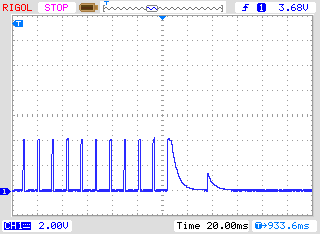
\includegraphics[]{../PNG/IRFU120gate.png}
\caption{Messung der Schwellspannung eines N-Kanal-MOSFET}
\label{fig:eleven}
\end{figure}

\subsection{Messung von Dioden}
\label{sec:diode}
Wenn Strom bei den Vortests festgestellt wurde, wird das Bauteil auf Diodenverhalten geprüft.
Die Flussspannung mit dem \(680\Omega\)-Widerstand muss zwischen 0,15V und 4,64V liegen.
Die Flussspannung mit dem \(680\Omega\)-Widerstand muss grösser als 1,125 Mal der Flussspannung mit dem
 \(470k\Omega\)-Widerstand sein und sechzehn Mal die Flussspannung mit dem \(470k\Omega\)-Widerstand muss
grösser als die Flussspannung mit dem \(680\Omega\)-Widerstand sein.
Zusätzlich darf die anschließende nochmalige Messung mit dem \(470k\Omega\)-Widerstand  keine höhere Spannung als die
Messung mit dem \(680\Omega\)-Widerstand ergeben.
Ich hoffe, dass ein Bauteil mit diesem Verhalten immer eine Diode ist.
Die Erkennung des Diodenverhaltens durch den fehlenden Stromfluß in der Gegenrichtung ist nicht
möglich bei antiparallelen Dioden.
Bei einer Einzeldiode wird zusätzlich der Sperrstrom der Diode bei 5V mit dem \(470k\Omega\) Widerstand
gemessen. Die Auflösung beträgt etwa \(2nA\). Bei größeren Restströmen als \(5.3\mu A\) (Spannung am Widerstand größer als 2.5V) wird
 mit dem \(680\Omega\) Widerstand gemessen. Dann beträgt die Auflösung nur etwa \(1\mu A\).
Außerdem wird bei Einzeldioden eine Kapazitätsmessung in Sperr-Richtung durchgeführt. 

\subsection{Ergebnisse der verschiedenen Messungen}
Die folgenden drei Tabelle zeigen die Ergebnisse verschiedener Bauteile 
eines ATmega8-Prozessors und verschiedenen Softwareversionen eines ATmega168-Prozessoren.
Die Messung der Sperrschichtkapazität für die Doppeldiode MBR4045PT gelingt
nur gekühlt. Die Ursache hierfür ist der hohe Reststrom der 40A Diode. Ebenso kann für die Basis - Emitter
Strecke des Germanium Transistors AC128 die Sperrschichtkapazität nur im
gekühlten Zustand gemessen werden. 

\begin{table}[H]
  \begin{center}
    \begin{tabular}{| l | c | c | c |}
    \hline
           & Mega8@8MHz          & Mega168 @8MHz       & Mega328 @8MHz     \\
 Diode Typ &                     &                     &                   \\
    \hline
    \hline
1N4148     & Diode, 715mV,        & Diode, 718mV,            & Diode, 715mV,           \\
           &               1pF    &               0pF, 2nA   &               1pF, 4nA  \\
    \hline
1N4150     & Diode, 665mV,        & Diode, 672mV,            & Diode, 666V,           \\
           &               1pF    &               1pF, 4nA   &              2pF, 6nA  \\
    \hline
BA157      & Diode, 619mV,        & Diode, 621V,              & Diode, 615mV,            \\
           &               19pF   &              17pF, 12nA   &               18pF, 12nA \\
    \hline
BY398      & Diode, 538mV,        & Diode, 541mV,             & Diode, 537mV,            \\
           &               16pF   &               14pF, 63nA  &               15pF, 63nA \\
    \hline
1N4007     & Diode, 650mV,        & Diode, 655mV,            & Diode, 650mV,           \\
           &               13pF   &               10pF, 6nA  &               13pF, 6nA \\
    \hline
LED green  & Diode, 1.96V, 5pF    & Diode, 1.95V, 4pF   & Diode, 1.95V, 4pF \\
    \hline
ZPD2,7     & 2xDi, 743mV, 2.53V   & 2xDi, 737mV, 2.52V  & 2xDi, 733mV, 2.51V \\
    \hline
BU508A B+E & Diode, 609mV,        & Diode, 611mV,                & Diode, 606mV,              \\
           &               5.15nF &               5.20nF, 0.39uA &               5.25nF, 0.4uA\\
    \hline
BU508A B+C & Diode, 582mV,        & Diode, 586mV,             & Diode, 587mV,            \\
           &               256pF  &               255pF, 21nA &               259pF, 19nA\\
    \hline
AC128 B+E  & Diode, 272mV,        & Diode, 277mV,              & Diode, 273mV,             \\
           &               0pF    &               0pF, 2.2uA   &               0pF, 2.3uA  \\
    \hline
AC128 B+E  &                      &                     & Diode, 349mV,               \\
gekühlt    &                      &                     &               140pF, 0.57uA \\
    \hline
MBR20100CT & 2xDi, 337mV, 337mV   & 2xDi, 338mV, 338mV  & 2xDi, 336mV, 335mV  \\
    \hline
MBR20100CT & Diode, 337mV,        & Diode, 339mV,             & Diode, 337mV,            \\
           &               345pF  &               351pF, 29nA &               350pF, 25nA\\
    \hline
MBR4045PT  & Diode, 243mV,        & Diode, 233mV,               & Diode, 235mV,              \\
gekühlt    &               1.80nF &               1.94nF, 1.7uA &               1.95nF, 1.8uA\\
    \hline
SF38G      & Diode, 519mV,        & Diode, 521mV,            & Diode, 516mV,            \\
           &               107pF  &               105pF, 2nA &               106pF, 2nA \\
    \hline
    \end{tabular}
  \end{center}
  \caption{Messergebnisse der Dioden-Tests}
  \label{tab:diodes} 
\end{table}

\begin{table}[H]
  \begin{center}
    \begin{tabular}{| l | c | c | c |}
    \hline
 Transistor & Mega8@8MHz          & Mega168 @8MHz       & Mega328 @8MHz    \\
    Typ     &                     &                     &                  \\
    \hline
    \hline
BU508A      & NPN, B=9, 602mV     & NPN, B=10, 594mV    & NPN, B=9, 591mV   \\
    \hline
2N3055      & NPN, B=20, 553mV    & NPN, B=22, 545mV    & NPN, B=21, 542mV  \\
    \hline
BC639       & NPN, B=180, 628mV   & NPN, B=215, 623mV   & NPN, B=173, 620mV \\
    \hline
BC640       & PNP, B=216, 635mV   & PNP, B=178, 635mV   & PNP, B=183, 600mV \\
    \hline
BC517       & NPN, B=26.1k, 1.20V & NPN, B=27.8k, 1.21V & NPN, B=26.1k, 1.20V\\
    \hline
BC516       & PNP, B=77.6k, 1.20V & PNP, B=81.1k, 1.19V & PNP, B=81.7k, 1.18V\\
    \hline
BC546B      & NPN, B=381, 659mV   & NPN, B=380, 653mV   & NPN, B=430, 675mV \\
    \hline
BC556B      & PNP, B=285, 689mV   & PNP, B=250, 688mV   & PNP, B=262, 654mV \\
    \hline
AC128 (Ge.) & PNP, B=63, 190mV    & PNP, B=61, 184mV    & PNP, B=59, 182mV  \\
    \hline
BRY55/200   & Thyristor           & Thyristor           & Thyristor        \\
    \hline
MAC97A6     & Triac               & Triac               & Triac        \\
    \hline
    \end{tabular}
  \end{center}
  \caption{Messergebnisse der Tests mit bipolaren Transistoren}
  \label{tab:bipolar} 
\end{table}

Die Ergebnisse unterscheiden sich teilweise erheblich von den Werten der Version 
von Markus Frejek. Zum Beispiel wird für den Darlington Transistor BC517 von
der früheren Software ein hFE von nur 797 statt 77600 gemessen. 
Dies hängt damit zusammen, dass die Stromverstärkung bei der neuen Version auch mit der
Kollektorschaltung gemessen wird.
Die Basis Emitter Spannung wurde früher mit einem separaten Diodentest mit 1438mV ermittelt.
Jetzt wird die angegebene Basis Emitter Spannung im Zustand der Verstärkungsmessung (1.20V) ermittelt.

In der folgenden Tabelle werden die Meßergebnisse von Germanium Transistoren gezeigt, die wegen den
stark Temperatur abhängigen Kollektor Restströmen besonders problematisch sind.
Es werden die Ergebnisse der Urversion von Markus F. und die Ergebnisse der aktuellen 1.08k Version
miteinander verglichen. Die 1.08k Version mißt mit dem ATmega328 die Stromverstärkung sowohl in der
Kollektorschaltung als auch in der Emitterschaltung, wobei die höhere Stromverstärkung ausgegeben wird.
Bei der 1.08k Version für den ATmega168 wird nur in der Kollektorschaltung gemessen.

\begin{table}[H]
  \begin{center}
    \begin{tabular}{| l | c | c | c |}
    \hline
 Transistor & Mega8@1MHz          & Mega168 @8MHz       & Mega328 @8MHz    \\
    Typ     & Ur-Version          & Version 1.08k       & Version 1.08k  \\
            & Markus F.           &                     &        \\
    \hline
    \hline
AC128       & PNP, B=52, 279mV    & PNP, B=61, 185mV    & PNP, B=60, 190mV    \\
    \hline
AC116-65    & PNP, B=505, 378mV   & PNP, B=56, 237mV    & PNP, B=76, 144mV    \\
    \hline
AC116-145   & PNP, B=485, 294mV   & PNP, B=83, 212mV    & PNP, B=167, 156mV   \\
    \hline
AC176-65    & NPN, B=98, 235mV    & NPN, B=52, 146mV    & NPN, B=57, 97mV     \\
    \hline
GC122       & PNP, B=84, 368mV    & PNP, B=56, 186mV    & PNP, B=58, 117mV    \\
    \hline
GC301       & PNP, B=48, 289mV    & PNP, B=40, 183mV    & PNP, B=40, 189mV    \\
    \hline
    \end{tabular}
  \end{center}
  \caption{Messergebnisse der Tests mit bipolaren Germanium Transistoren}
  \label{tab:germanium} 
\end{table}

\begin{table}[H]
  \begin{center}
    \begin{tabular}{| l | c | c | c |}
    \hline
             & Mega8@8MHz       & Mega168 @8MHz    & Mega328 @8MHz \\
 FET Typ     &                  &                  &               \\
    \hline
    \hline
ZVNL120A     & N-E-MOS,D, 1.6V  & N-E-MOS,D, 1.5V  & N-E-MOS,D, 1.5V \\
             & 147pF            & 139pF            & 140pF \\
    \hline
IRF530N      & N-E-MOS,D, 3.6V  & N-E-MOS,D, 3.6V  & N-E-MOS,D, 3.6V \\
             & 1.55nF           & 1.54nF           & 1.56nF \\
    \hline
BS170        & N-E-MOS,D, 2.6V  & N-E-MOS,D, 2.6V  & N-E-MOS,D, 2.6V \\
             &  78pF            &  68pF            &  70pF \\
    \hline
IRL3803      & N-E-MOS,D, 2.3V  & N-E-MOS,D, 2.3V  & N-E-MOS,D, 2.3V \\
             & 9.81nF           & 9.71nF           & 9.80nF \\
    \hline
IRFU120N     & N-E-MOS,D, 4.2V  & N-E-MOS,D, 4.2V  & N-E-MOS,D, 4.2V \\
             & 909pF            & 913pF            & 920pF \\
    \hline
BUZ71A       & N-E-MOS,D, 3.2V  & N-E-MOS,D, 3.2V  & N-E-MOS,D, 3.2V \\
             & 714pF            & 708pF            & 714pF \\
    \hline
ZVP2106A     & P-E-MOS,D, 3.2V  & P-E-MOS,D, 3.2V  & P-E-MOS,D, 3.2V \\
             & 122pF            & 115pF            & 117pF \\
    \hline
IRF5305      & P-E-MOS,D, 3.6V  & P-E-MOS,D, 3.6V  & P-E-MOS,D, 3.6V \\
             & 2.22nF           & 2.22nF           & 2.24nF \\
    \hline
BS250        & P-E-MOS,D, 2.6V  & P-E-MOS,D, 2.6V  & P-E-MOS,D, 2.6V \\
             & 53pF             & 43pF             & 44pF \\
    \hline
IRFU9024     & P-E-MOS,D, 3.5V  & P-E-MOS,D, 3.6V  & P-E-MOS,D, 3.5V \\
             & 937pF            & 945pF            & 952pF \\
    \hline
J310         & N-JFET           & N-JFET           & N-JFET\\
Idss=24-60mA & I=3.1mA Vgs=2.2V & I=3.1mA Vgs=2.2V & I=3.1mA Vgs=2.2V \\
    \hline
2N5459       & N-JFET           & N-JFET           & N-JFET\\
Idss=4-16mA & I=2.1mA Vgs=1.5V & I=2.1mA Vgs=1.5V & I=2.1mA Vgs=1.5V \\
    \hline
BF256C       & N-JFET           & N-JFET           & N-JFET\\
Idss=11-18mA & I=3.4mA Vgs=2.4V & I=3.4mA Vgs=2.4V & I=3.4mA Vgs=2.4V \\
    \hline
BF245A       & N-JFET           & N-JFET           & N-JFET\\
Idss=2-6mA   & I=1.1mA Vgs=.75V & I=1.1mA Vgs=0.75V & I=1.1mA Vgs=0.75V \\
    \hline
BF245B       & N-JFET           & N-JFET           & N-JFET\\
Idss=6-15mA  & I=2.5mA Vgs=1.7V & I=2.5mA Vgs=1.7V & I=2.5mA Vgs=1.7V \\
    \hline
BF245C       & N-JFET           & N-JFET           & N-JFET\\
Idss=12-25mA & I=3.9mA Vgs=2.7V & I=3.9mA Vgs=2.7V & I=3.9mA Vgs=2.7V \\
    \hline
J175        & P-JFET           & P-JFET           & P-JFET\\
Idss=7-60mA & I=3.2mA Vgs=2.2V & I=3.2mA Vgs=2.2V & I=3.2mA Vgs=2.2V \\
    \hline
2N5460      & P-JFET           & P-JFET           & P-JFET\\
Idss=1-5mA  & I=0.78mA Vgs=0.54V & I=0.77mA Vgs=0.54V & I=0.78mA Vgs=0.54V \\
    \hline
    \end{tabular}
  \end{center}
  \caption{Messergebnisse der MOS-Transistor-Tests}
  \label{tab:mos} 
\end{table}
